We illustrate the subset selection method with a case study assessing the seismic risk to the San Francisco Bay Area highway and local road network, as measured by the change in morning commute travel time for the 9-county region's approximately 7 million people~\cite{carr_study_2007}. 

\subsection{Dataset and models}

\subsubsection{Ground-motion intensity map models}

To generate a stochastic catalog of ground-motion intensity maps, we use the OpenSHA Event Set Calculator~\cite{field_opensha:_2003}. This software outputs the mean, $\overline{\ln Y_{ij}}$, and standard deviation values, $\sigma_{ij}$ and $\tau_j$, for all locations of interest for a specified seismic source model and ground motion prediction equation. The intensity measure is the 5\%-damped pseudo absolute  spectral acceleration ($Sa$) at a period $T=1s$, which is the required input to the fragility functions below. While our results use spectral acceleration, other intensity measures could be used to characterize the ground motion as long as a corresponding ground motion prediction model and spatial correlation model are available~\cite[e.g.,][]{foulser-piggott_predictive_2012}. %e.g., Foulser-Piggott and Stafford 2011). 
We use the UCERF2 seismic source model~\cite{field_uniform_2009}, Wald and Allen topographic slope model for the the shear wave velocity $V_{s30,i}$~\cite{wald_topographic_2007}, and the Boore and Atkinson \cite{boore_ground-motion_2008} ground motion prediction equation.   Using this seismic source model, which is then discretized into a list of faults and a stratified list of magnitudes and rupture locations for each, we obtain a set of 2110 earthquake events on active faults, and with annual occurrence rates greater than or equal to $10^{-5}$.


We simulate the baseline set of maps by combining the mean terms from the Event Set Calculator and spatially-correlated residual terms of the ground-motion intensity  (using~\cite{jayaram_correlation_2009}) according to the basic ground motion model~\eqref{eq:GMPE}. The baseline set has 5 residual realizations per ground motion scenario, which results in 10,550 ground-motion intensity maps (e.g., Figure~\ref{fig:sample_pipeline}{\color{red}(a)}).  We also generate two smaller sample sets of candidate ground-motion intensity maps that will be inputs to the optimization problem: one set with one residual realization per ground motion scenario (2110 maps total) and another with two residual realizations per ground motion scenario (4220 maps total). These two sets represent computationally-feasible set sizes for the optimization problem, and also enable testing the sensitivity of the optimization results to the input set size.

\subsubsection{Damage maps}%Description of network and its components} %includes bridge fragility and people exposure
We use a portfolio of 1743 highway bridges in the San Francisco Bay Area, which includes all unique state-managed bridges in current operation on the road network (illustrated in Figure~\ref{fig:sample_pipeline}{\color{red}(b)}). The bridges were hand-matched to road segments in the case study network (major roads illustrated in Figure~\ref{fig:sample_pipeline}{\color{red}(c)}).  If a bridge collapses, the road segment it carries, as well as that which it crosses, are modeled as closed. We do not include other types of failures, such as road damage from liquefaction, that may damage the network.

%We do not include other types of network component failures such as liquefaction in this study.

To compute damage to the bridges, we use fragility functions of the following form:
\begin{equation}
%$P(DS \geq ds_s | Y = y_{ij'}, i)$
P(DS_i \geq ds_s |Y_{ij} = y) = \Phi \left( \frac{\ln y - \lambda_{s, i}}{\xi} \right),
\label{eq:dsfull}
\end{equation}
where $\Phi$ is the standard normal cumulative distribution function, $\lambda_{s,i}$ and $\xi$ are respectively the mean and standard deviation of the $\ln Y$ value necessary to cause the $s^{th}$ damage state to occur or be exceeded, and $y$ is a realization of the random variable $Y_{ij}$, the ground-motion intensity at the $i^{th}$ site and $j^{th}$ ground-motion intensity map. The other variables are defined above.


The California Department of Transportation (Caltrans) provided the fragility function values $\lambda_{s,i}$ and $\xi$ used in this study. The values are based on structural characteristics including number of spans and structure age as detailed in \cite{basoz_enhancement_1999}.
%
% using the method detailed in \cite{basoz_enhancement_1999} based on The structural capacities of individual bridges are modeled as uncorrelated.

Per ground-motion intensity map, we compute one damage map (e.g., Figure~\ref{fig:sample_pipeline}{\color{red}(b)}), which has a realization of the bridge damage state at each bridge location according to the fragility function~\eqref{eq:dsfull}. The provided fragility functions do not consider correlation of the bridge capacities, but other models could be used~\cite[e.g.,][]{baker_introducing_2008}.

Each bridge damage state maps directly to the traffic capacity on associated road segments. We represent the road network by a directed graph $G = (V, E)$, where $V$ is a finite set of vertices representing intersections and the set $E$, whose elements are edges representing road segments, is a binary relation on $V$. Some edges (road segments) are matched to bridges, as described above. This study considers the Metropolitan Transportation Commission (MTC) \emph{Travel Model One} (version 0.3) of the San Francisco Bay Area transportation network where $(|V|, |E|) = (11921, 32858)$ including centroidal road segments and $(|V|, |E|) = (9635, 24404)$ without. Centroidal links refer to links that do not correspond to particular physical roads, but instead capture more subtle traffic flows, such as  from outside the study area, or the traffic flow to and from some minor local roads. The model includes both highways and main local roads as well as the relevant trip demand data. The travel origin-demand matrix for the latest run version, 2010\_03\_YYY, is from the MTC and is divided based on population density into 34 super districts covering the 9-county San Francisco Bay Area.

We use a functional percentage relationship to compute the traffic capacity of relevant road segments. Based on discussions with Caltrans, we consider travel conditions one week after an earthquake, since it is a critical period for decision making. For example, one week after most events, bridges should have been inspected and surface damage should be repaired, but major reconstruction would not have yet begun. According to our functional percentage relationship, at this point in time, the bridges have one of two classes of functionality, zero traffic capacity and full traffic capacity~\cite{werner_redars_2006}. We can thus summarize the bridge damage using two damage states $ds_s$, $ds_{damaged}$ and $ds_{functional}$, which correspond to the common HAZUS \emph{extensive} or \emph{complete} damage states and the \emph{none}, \emph{slight}, or \emph{moderate} damage states respectively~\cite{werner_redars_2006}. Thus, the functional percentage relationship assigns zero traffic capacity on road segments that have at least one bridge in the $ds_{damaged}$ damage state, and full traffic capacity otherwise. 



\subsubsection{Target network performance measures}\label{sec:perf}
We select the average change in morning commute time under fixed travel demands, which is proportional to the commonly-used fixed-demand travel delay for the same time period, as our target network performance measure. The morning commute time period is defined as 6am to 10am on weekdays. 

We estimate the trip time with the iterative traffic assignment (ITA) method \cite{chen_network_1991}, which has been shown by \cite{wang_understanding_2012} to be consistent with results from the commonly-used User Equilibrium (UE) method and to better estimate driver behavior because intuitively it captures drivers' choices of routes based on what traffic situation they currently see. We implement ITA according to the recommendations of \cite{wang_understanding_2012}  where the original demand matrix is divided into four parts, with 40\%, 30\%, 20\%, and 10\% respectively of the total trips. To begin, the first part of the trips are assigned using Dijkstra's algorithm to find shortest paths where the non-negative edge weights are the free-flow travel time ($t_f$). The resulting link flows ($q_f$) are recorded for each link. Then, we update the travel time ($t_a$) on each link according to the commonly-used formula, 
\begin{equation}
t_a = t_f \left( 1 + 0.15 \left( \frac{q_f}{c_f}\right)^{4}\right),
\end{equation}
where $c_f$ is the flow capacity of the link and the other variables are defined above~\cite{bureau_of_public_roads_traffic_1964}. Thus, travel time is a quartic function with link flow. Then, using these new free-flow times ($t_a$) as the edge weights, we use Dijkstra's algorithm to assign the second part of the trips. We repeat this approach until we have assigned all four parts of the trips.

We implement ITA in Python by leveraging the Python network analysis module NetworkX~\cite{hagberg_exploring_2008} (with some base algorithms in C and FORTRAN). The final result is a target performance measure and corresponding map (e.g., Figure~\ref{fig:sample_pipeline}{\color{red}(c)}) per ground-motion intensity map.

\subsubsection{Proxy network performance measures}
We now describe the selection of an appropriate proxy performance measure that is computationally inexpensive yet correlated with the target performance measure. We could select the performance measure by computing empirical correlation between the target and each candidate proxy measure for a computationally tractable number of scenarios. Another complementary strategy is to use other knowledge about the problem dynamics, such as in this case that the travel time should be related to bridge damage since the only network damage we are considering is directly related to bridges in a damaged state.  

To select a proxy performance metric for the case study, we randomly choose 10 ground-motion intensity maps and corresponding damage maps. For each damage map, we compute the values of the following candidate proxy performance measures: percent of bridges damaged, percent reduction in traffic flow capacity, and weighted-shortest path between locations of interest. 
%To select a proxy performance metric for the case study, we choose a set of 10 ground-motion intensity maps and corresponding damage maps for each for a group of candidate proxy performance measures, namely percent of bridges damaged, percent reduction in traffic flow capacity, and weighted-shortest path between locations of interest. 
To illustrate sensitivity to the initial set of scenarios, we provide the empirical $95^{th}$ percentile (point-wise) confidence interval by generating 100 realizations of 10 maps, sorting the empirical correlation values, and displaying the $5^{th}$ and $95^{th}$ percentile values (as well as the median) (Figure~\ref{fig:rhos}).  We find that \emph{percent of bridges damaged} is the proxy performance measure that across different quantiles on the confidence interval is most correlated with the target measure, which is corroborated by our engineering judgement. 
While we have provided the confidence interval to show the relative robustness of the method, it would not be calculated in practice because it is computationally expensive (namely requiring 100 sets of 10 evaluations of the target performance metric). We find that choosing just 10 random ground-motion intensity values and testing empirical correlation values provides insight into which proxy performance metric will be representative of the target performance metric. However, given some variability, particularly below the $50^{th}$ percentile values, this quantitative test should be supplemented with engineering judgement as described above. 


\begin{figure}[t!]
\centering
\includegraphics[width=3.75in]{../FIGS/subsets_rho.eps} 
\caption{Median (black dots) and empirical $95^{th}$ percentile point-wise confidence interval of the empirical correlation coefficient between candidate proxy performance measures and the target performance measure. Percent of bridges damaged is most highly correlated.}
\label{fig:rhos}
\end{figure}



\subsection{Map selection results and checks for consistency}
In this section, we select the optimization parameters, describe the resulting final subset of ground motion and damage maps, and then check the consistency of the results with the ground-motion intensity and performance measure rates of exceedance. 

\subsubsection{Final map selection} \label{sec:finalresults}
The optimization problem is solved using CVX, a Matlab package for specifying and solving convex problems \cite{grant_cvx:_2012, grant_graph_2008}, with the Gurobi Optimizer~\cite{gurobi_optimization_gurobi_2013}, for linear and mixed integer programming. We select maps using both the original nonconvex problem and the relaxed problem using convex constraints to compare their performance. The optimization problem~\eqref{eq:optim} is solved using a linear programming-based parallel branch and bound algorithm. The solver terminates (with an optimal result) when the gap between the lower and upper bounds of the objective function is less than 0.1\% of the upper bound~\cite{gurobi_optimization_gurobi_2013} or after 30 million iterations, whichever occurs first. Thus, in the numerical experiments here, the problem is solved using heuristics based on convex optimization. The relaxed problem using convex constraints~\ref{eq:optim} is also solved using CVX with the Gurobi Optimizer and terminates when an optimal solution is found. Supplementary information about the final map selection can be found in Appendix D of~\cite{miller_seismic_2014}. Furthermore, to facilitate adoption of the proposed methodology, Matlab implementations of both optimization-based map-selection methods are available at \href{http://purl.stanford.edu/wq017yv5965}{http://purl.stanford.edu/wq017yv5965}.

Next we set the relevant optimization parameters. In addition to the termination criteria, we have five main parameters to choose: the relative importance of ground-motion intensity versus the performance measure ($\alpha$), the number of return periods ($R$), the number of sites at which the objective function will be minimized ($\nu$), the number of candidate damage maps and corresponding ground-motion intensity maps ($J$ in general, which equals $m$ for the case study since $c=1$), and the desired number of ground-motion intensity maps in the final subset ($k$). 

We choose $k=25$ maps as a near-lower-bound case of the number of maps selected. In Section~\ref{sec:discussOpt} we will show results where $k=200$ maps for comparison with prior work.
% ($\frac{k}{2m + 2R(1+n)} < 0.02$ in the authors' experience)
With a small number of maps desired in the subset compared to the number of random variables, which is the case when $k=25$, we find that the alternative optimization formulation using convex constraints performs poorly. Since that method selects the scenarios with the $k$ highest renormalized annual rates, it excludes rare high intensity events, in practice, when the total number of maps ($k$) is very small. So, for the results below, we will use the original formulation~\eqref{eq:optim}. 

%However, when $k=200$ maps, we will show that near-identical subsets are selected using the original optimization problem and the alternative with convex constraints. Furthermore, the alternative finishes in a fraction of the time (hundredths of a second versus 70 seconds on a 2.8GHz desktop computer using the final parameters) and the result is guaranteed to be optimal.

We then determine the $\alpha, R, \nu$ and $J$ values empirically using grid search and computing the value of an evaluation function for each parameter combination (to ensure like comparisons, the evaluation function is $0.5$ MHCE $+ 0.5$ MPMCE(proxy) with 1743 sites and 50 return periods).  Grid search is a standard way of selecting parameters by exhaustively searching through a manually-specified subset of the parameter space. Note that while it may seem beneficial to use large values for $R, \nu$ and $J$, increasing the number of random variables makes convergence more challenging and can thus potentially increase error. Furthermore, there can be overfitting that causes MPMCE(target) to increase even as the objective function value decreases.


Via grid search, we determine our final set of parameters: $(\alpha, R, \nu, J, k) = (0.56, 50, 12, 2110, 25)$. The result of the original optimization problem~\eqref{eq:optim} using these parameters is the final output:  25 damage maps, corresponding ground-motion intensity maps, and associated annual occurrence rates. 

We will use this subset as an illustration; other subsets could have been selected with a different choice of parameter values or convergence criteria.  Furthermore, since computational time depends on the number of random variables, we find that in general, the choice of $J$ should capture, at least, the basic distribution of earthquake scenarios. The other parameter values can be explored using the grid search approach above, which we illustrated further in~\cite{miller_framework_2014}; one should include higher values in the parameter space (and thus a higher number of random variables), while the computation is feasible. Finally, note that the consistency checks below also help with tuning the parameters. This allows for leveraging any additional user expertise not  captured in the optimization formulation.


\subsubsection{Consistency checks}
We perform five checks: four  to evaluate how well the chosen set of ground-motion intensity maps and adjusted annual rates of occurrence represents the full joint distribution of $Sa$, and then one to test how well the selected subset and rates represent the baseline set of exceedance rates of the proxy performance measure.

%\renewcommand{\theenumi}{\Roman{enumi}}
\begin{enumerate}
\item \textbf{Fault sources} A possible pitfall is to primarily include events stemming from a major fault, such as the San Andreas Fault. In contrast, our subset still contains a range of faults, with no single fault contributing to more than 50\% of the annual rate of occurrence. Furthermore, since we constrain the ground-motion intensity maps inputted to the optimization to those with an annual occurrence rate of at least $10^{-5}$, we automatically have reasonably active faults in the final subset. 
\item \textbf{Magnitudes}  When we investigate the distribution of magnitudes, we see that the subset underestimates the rates at particularly low magnitudes. This behavior is not surprising because we have chosen to only match the exceedance curves between rates of 0.01 and 0.004 (return periods of 100 to 2500 years) and the low magnitude events are often more frequent, thus outside of the target range. However, there is a general good correspondence~\cite{miller_framework_2014}.

\item \textbf{Marginal distributions of ground-motion intensities} After looking at magnitudes, we compare the ground-motion intensity exceedance curves at individual sites. We compare results at two sites where the main contributors to the hazard are expected to be different  (Figure~\ref{fig:distributions}{\color{red}(c)}). The exceedance curves from the subset  fit reasonably well with the results from the baseline set, particularly between the return periods of 100 and 2500 years (e.g., Figure~\ref{fig:distributions}{\color{red}(a,d)}). This qualitative verification is corroborated by our overall error metric MHCE value~\eqref{eq:MHCE}, which averaged over all sites and 50 return periods is 30.3\%. For determining the size of a randomly-chosen set that, on average, gets the same error, readers can randomly select different size sets of ground-motion intensity maps and damage maps, normalize the $w_{j'}$, compute the error metrics, and compare~\cite{gearhart_optimization-based_2014}.
\item\textbf{Joint distributions of ground-motion intensities} 
The optimization has not explicitly considered the consistency of multivariate ground motion distributions when selecting the subset of maps.
However, we find that the realizations from the chosen subset and the baseline set are plausible pairings (Figure~\ref{fig:distributions}{\color{red}(b)}).
%It is not obvious that a stochastic catalog of ground-motion intensity maps that appear individually representative of different sites would still appear reasonable when considering a joint distribution. 
%However, we find that the empirical distribution from the subset relatively accurately defines the results from the extensively-sampled set, including skew (how balanced the distribution is on each side of the mean) and correlation (tightness of the simulation results band). 
This trend even appears for two sites where we might expect poor results because they have very different contributions to their ground motion hazard (Hayward Fault and San Andreas Fault, respectively, having major contributions). Thus, the results suggest that the optimization problem implicitly considers joint ground motion behavior because of the combination of minimizing error at each location individually and minimizing error to a region-wide metric that depends on joint bridge damage, and thus joint ground-motion intensities.
\item \textbf{Proxy performance measure} We see that the exceedance curve of the proxy performance measure~\eqref{eq:exceedance} using the selection results described in Section \ref{sec:finalresults} reasonably fits the exceedance curve of the baseline set (Figure~\ref{fig:pm}{\color{red}(a)}). This result corresponds to the summary error value of MPMCE(proxy) $= 7.1\%$ over 50 return periods and all 1743 locations. We do see that the subset underestimates the risk at return periods less than 100 years, which is outside the range of interest for the case study. If these return periods were of interest, then the return period parameters in the optimization could be adjusted accordingly.
\end{enumerate}
If the results are not as consistent for another application, one might try adjusting the parameters, for example, decreasing $\alpha$ to increase the contribution of fitting the marginal distributions of the ground-motion intensities in the objective function (or vice versa for the opposite effect), or increasing the total number of maps ($k$) used in the optimization. As the number of random variables is increased, one may also need to increase the relative gap and/or increase the maximum number of iterations associated with optimization termination. Thus, by following this step-by-step procedure and making any necessary adjustments, the modeler can be reasonably confident of the representativeness of the chosen subset for a seismic risk assessment of an infrastructure network.

\subsubsection{Target performance measure results}
Although the goal of the proposed selection procedure is to save computational time by not evaluating the target performance measure for the baseline set, for illustration, we will now compare results between the selected subset and the baseline set to test our set result. We find that the selected subset (ground-motion intensity maps, corresponding damage maps and occurrence rates) produces a reasonable estimate (Figure~\ref{fig:pm}{\color{red}(b)}). This corresponds to MPMCE(target) $= 2.7\%$ over 50 return periods. Also, as for the proxy measure, we observe that the estimate is most accurate within the return periods of interest included in the optimization. It may not be immediately obvious why MPMCE(target) is lower than MPMCE(proxy). This behavior stems from the definition of MPMCE that involves a sum of normalized differences in the performance metric between the exceedance curve from the baseline set compared to the exceedance curve from the selected subset (Section \ref{sec:errors}). The proxy metric has a larger range of values in the return periods of interest than the target metric so it comparably fares worse (Figure~\ref{fig:pm}). For example, if we instead include the target metric in the optimization formulation and test the subset on the proxy metric, we find that the error on the target metric decreases (since it is included in the optimization and it inherently has a lower range of values in the return periods of interest) while the error on the proxy metric increases (since it is not included in the optimization and there is a large range of values in the range of the return periods of interest). In conclusion, we see that the target performance measure results have relatively low error, even when the subset of damage maps is chosen only by the proxy performance measure and ground-motion intensity.
 

\begin{figure}[t!]
\centering
\includegraphics[width=5.6in]{../FIGS/subsets_distributions.eps} %subset_joints.pdf}
\caption[]{Ground-motion intensity exceedance curve comparison between the subset of ground-motion intensity maps where $k=25$ and the baseline set: (a) marginal exceedance curve at site B, (b) bivariate exceedance curve at sites A and B, (c) study map showing locations of sites A and B, and (d) marginal exceedance curve at site A. The grey box in panels (a) and (d) mark the range of the return periods of interest. }
\label{fig:distributions}
\end{figure}



\begin{figure}[t!]
\centering
\includegraphics[width=5.6in]{../FIGS/subsets_pm.eps} %subset_pm.pdf}
\caption{Comparison of the performance measure exceedance curves between the subset of ground-motion intensity maps where $k=25$ and the baseline set for (a) the proxy performance measure (percentage of bridges damaged), and (b) the target performance measure (percentage change in morning commute time). The grey box marks the range of return periods of interest.}
\label{fig:pm}
\end{figure}


